\documentclass{beamer}
\usepackage{graphicx}
\usepackage{grffile}
\usepackage{mathtools}
\usepackage{amssymb}
\usepackage{multicol}
\usepackage{url}
\usetheme{CambridgeUS}


\title[]
{Classification of Finite Simple Groups}
\author
{Adam Michael}
\institute[Rose-Hulman]
{
	MA376 - Abstract Algebra\\
	Department of Mathematics\\
	Rose-Hulman Institute of Technology
}
\date[May 9, 2016]
{May 9, 2016}
\subject{Topology}

\beamertemplatenavigationsymbolsempty


\begin{document}
\frame{\titlepage}

\begin{frame}
	\frametitle{Simple Groups}
	\begin{definition}
	A simple group is a nontrivial group with no normal subgroups aside from itself and the trivial group.
	\end{definition}
\end{frame}

\begin{frame}
	\frametitle{Galois Theory sparked the study of finite simple groups} 
	\begin{definition}
	A group $G$ is solvable if there is a chain of subgroups $\{e\} = G_0 \triangleleft G_1 \triangleleft ... \triangleleft G_k = G$ such that each $G_i / G_{i-1}$ is abelian \cite{gallian}.
	\end{definition}
	\begin{examples}
	\begin{itemize}
		\item
		If $G$ is abelian, then $\{e\} \triangleleft G$, $G/\{e\}$ is abelian, so $G$ is solvable.
		\item
		$\{e\} \triangleleft A_3 \triangleleft S_3$, $A_3/ \{e\} \cong A_3 \cong \mathbb{Z}_3$, $S_3/A_3 \cong \mathbb{Z}_2$ so $S_3$ is solvable.
		\item
		If $G$ is a nonabelian simple group, then $G$ is not solvable.
	\end{itemize}
	\end{examples}
	\begin{theorem}
	A polynomial is solvable by radicals if and only if its ``Galois group'' is solvable.
	\end{theorem}
\end{frame}

\begin{frame}
	\frametitle{Classification of Abelian Finite Simple Groups}
	\begin{theorem}
	A finite abelian group $G$ is simple if and only if $G \cong \mathbb{Z}_p$ for some prime $p$.
	\end{theorem}
	\begin{proof}
	By LaGrange's Theorem, $\mathbb{Z}_p$ is simple. By the Fundamental Theorem of Finite Abelian Groups, $G \cong \mathbb{Z}_{{p_1}^{e_1}} \times ... \times \mathbb{Z}_{{p_k}^{e_k}}$. If $k > 1$, $G$ has a normal subgroup isomorphic to $\mathbb{Z}_{{p_1}^{e_1}}$. If $k = 1$ and $e_1 > 1$, $G$ has a normal subgroup isomorphic to $\mathbb{Z}_{{p_1}}$.
	\end{proof}
\end{frame}

\begin{frame}
	\frametitle{Conjugate Subgroups}
	\begin{definition}
	For subgroups $H_1$ and $H_2$ of $G$, $H_1$ is conjugate to $H_2$ if there exists a $g \in G$ such that $g H_1 g^{-1} = H_2$.
	\end{definition}
		\begin{theorem}
	If $H \le G$, $H$ is normal if and only if $H$ has no conjugates in $G$.
	\end{theorem}
	\begin{proof}
		\begin{enumerate}
			\item[$\Rightarrow$]
			Let $H \triangleleft G$. Then $\forall g \in G$, $g H g^{-1} = H$, so $H$ has no conjugates.
			\item[$\Leftarrow$]
			Let $H_1 \ntriangleleft G$. Then $\exists g \in G$ such that $g H_1 g^{-1} \ne H_1$. Let $H_2 = \{g h g^{-1} | h \in H_1\}$. Consider $g h_1 g^{-1}, g h_2 g^{-1} \in H_2$. Then $g h_1 g^{-1} (g h_2 g^{-1})^{-1} = g (h_1 h_2^{-1}) g^{-1} \in H_2$. So $H_2 \le G$ by the 1 Step Subgroup Test. So $H_1$ is conjugate to $H_2$ and $H_1 \ne H_2$.
		\end{enumerate}
	\end{proof}
\end{frame}

\begin{frame}
	\frametitle{Sylow Theorems}
	\begin{theorem}[Sylow Theorems \cite{wilson}, 1872]
	If $G$ is a finite group of order $p^k n$, $p$ prime and $p \nmid n$, then
	\begin{enumerate}
		\item $G$ has $s_p \ge 1$ subgroups of order $p^k$, called Sylow $p$-subgroups
		\item The Sylow $p$-subgroups are all conjugate
		\item $s_p \mid m$ and $s_p \equiv 1 \mod p$	
	\end{enumerate}
	\end{theorem}
	\begin{example}
	If $s_p = 1$ then the Sylow $p$-subgroup is normal so $G$ is not simple.
	\end{example}
\end{frame}

\begin{frame}
	\frametitle{Feit-Thompson Theorem}
	\begin{theorem}[Feit-Thompson Theorem \cite{wilson}, 1962]
	Every finite group of odd order is solvable.
	\end{theorem}
	\begin{corollary}
	Every nonabelian finite simple group has even order.
	\end{corollary}
\end{frame}

\begin{frame}
	\frametitle{The Classification Theorem for Finite Simple Groups \cite{wilson}}
	\begin{theorem}[The Classification Theorem for Finite Simple Groups \cite{wilson}, 2004]
	Every finite simple group is isomorphic to one of the following:
	\begin{itemize}
	\item
	The cyclic groups $\mathbb{Z}_p$ for prime $p$
	\item
	The alternating groups $A_n$ for $n \ge 5$
	\item
	The classical groups of Lie type
	\item
	The exceptional groups of Lie type or the Tits group ${}^2F_4(2)'$
	\item
	26 sporadic finite simple groups		
	\end{itemize}
	\end{theorem}
\end{frame}

\begin{frame}
	\frametitle{Classical Groups of Lie Type}
	For a prime-power $q$,
		\begin{itemize}
		\item
		Linear: $PSL_n(q)$, $n \ge 2$, except $PSL_2(2)$ and $PSL_2(3)$
		\item
		Unitary: $PSU_n(q)$, $n \ge 3$, except $PSU_3(2)$
		\item
		Symplectic: $PSp_{2n}(q)$, $n \ge 2$, except $PSp_4(2)$
		\item
		Orthogonal:
		\begin{itemize}
			\item
			$P\Omega_{2n+1}(q)$, $n \ge 3$, $q$ odd
			\item
			$P\Omega^+_{2n}(q)$, $n \ge 4$
			\item
			$P\Omega^-_{2n}(q)$, $n \ge 4$
		\end{itemize}
	\end{itemize}
	\begin{example}
		$PSL_n(q) = SL_n(q) / Z$ where $SL_n(q)$ is the group of $n \times n$ matrices with entries from the finite field $\mathbb{F}_q$ with determinant 1 and $Z$ is the subgroup of $SL_n(q)$ that are scalar multiples of the identity \cite{wilson}.
	\end{example}
\end{frame}

\begin{frame}
	\frametitle{Exceptional Groups of Lie Type}
	For a prime-power $q$,
	\begin{multicols}{2}
	\begin{itemize}
		\item $G_2(q)$, $q \ge 3$ ;
		\item $F_4(q)$;
		\item $E_6(q)$;
		\item ${}^2E_6(q)$;
		\item ${}^3D_4(q)$;
		\item $E_7(q)$;
		\item $E_8(q)$
		\item ${}^2B_2(2^{2n+1})$, $n \ge 1$;
		\item ${}^2G_2(3^{2n+1})$, $n \ge 1$;
		\item ${}^2F_4(2^{2n+1})$, $n \ge 1$
	\end{itemize}
	\end{multicols}
\end{frame}

\begin{frame}
	\frametitle{Sporadic Finite Simple Groups}
	\begin{itemize}
		\item
		The Mathieu groups $M_{11}, M_{12}, M_{22}, M_{23}, M_{24}$
		\item
		The Leech lattice groups $Co_1, Co_2, Co_3, McL, HS, Suz, J_2$
		\item
		The Fischer groups $Fi_{22}, Fi_{23}, Fi'_{24}$
		\item
		The monstrous groups $\mathbb{M}, \mathbb{B}, Th, HB, He$
		\item
		The pariahs $J_1, J_3, J_4, O'N, Ly, Ru$.
	\end{itemize}
\end{frame}

\begin{frame}
	\frametitle{Sporadic Finite Simple Groups}
	\begin{definition}
		If $G$ is a group and $N \triangleleft H \le G$, then $H / N$ is called a subquotient of $G$ \cite{dummit}.
	\end{definition}
	\begin{figure}
		\centering
		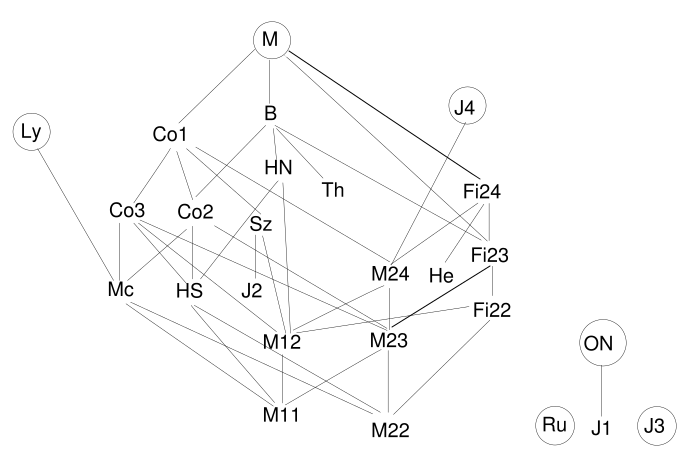
\includegraphics[height=140pt,keepaspectratio]{monstergroupdiagram}
		\caption{Subquotient diagram of sporadic finite simple groups \cite{monsterdiagram}}
	\end{figure}
\end{frame}

\begin{frame}
	\frametitle{References}
	\bibliographystyle{ieeetr}
	\bibliography{bibliography}
\end{frame}
\end{document}